\documentclass[a4paper,12pt]{article}

% Packages
\usepackage[utf8]{inputenc}
\usepackage{geometry}
\usepackage{titlesec}
\usepackage{lipsum} % for generating dummy text
\usepackage{graphicx}
\usepackage{caption}
\usepackage{subcaption}
\usepackage{listings}
\usepackage{amsmath}
\usepackage{amssymb}                                                                                                                                                            
\usepackage{xcolor}

% Page setup
\geometry{a4paper, margin=1in}
\setlength{\parindent}{0pt}
\setlength{\parskip}{5pt}

% Title setup
\title{\textbf{DSP LAB - Experiment 4} \\
    \large{Fixed and Floating Point Convolution and Correlation}}                                                       
\author{Ajay Krishnan K \\  EE22BTECH11003}
\date{\today}

% Section and subsection formatting
\titleformat{\section}[block]{\normalfont\Large\bfseries}{\thesection}{1em}{}
\titleformat{\subsection}[block]{\normalfont\large\bfseries}{\thesubsection}{1em}{}
\titleformat{\subsubsection}[block]{\normalfont\normalsize\bfseries}{\thesubsubsection}{1em}{}

% Code listing settings
\lstdefinestyle{mystyle}{
    language=Matlab,
    basicstyle=\ttfamily\small,
    breaklines=true,
    keywordstyle=\color{blue},
    commentstyle=\color{green!40!black},
    stringstyle=\color{red},
    % numbers=left,
    % numberstyle=\tiny,
    frame=single,
    showspaces=false,
    showstringspaces=false,
}

\lstset{style=mystyle}

\begin{document}
\maketitle

\tableofcontents

\newpage

\section{Aim}
To implement fixed and floating point convolution and correlation in MATLAB and C and compare the results
by calculating the mean square of the difference between the fixed and floating point results and
 plotting the square of the difference.

\section{Theory}
\subsection{Convolution}
Convolution is a mathematical operation on two functions (f and g) to produce a 
third function that expresses how the shape of one is modified by the other. 
The term convolution refers to both the result function and to the process of computing it.
 In discrete time, the convolution of two sequences is given by
\[
    y[n] = \sum_{k=-\infty}^{\infty} x[k]h[n-k]
\]

\subsubsection{Implementation in MATLAB}
First, both the sequences are converted to fixed point using the custom floatToFixed function 
and then the convolution is performed using the convtaker function. Then qFactor multiplied fixed point array
is converted back to fixed point by dividing by ${(qFactor)}^2$. Then the absolute square difference and mean square error is calculated.
Subsequently, the absolute square of the difference between the fixed and floating point results is plotted.

\subsubsection{Matlab Code}
\lstinputlisting[language=Matlab]{../code/convolution.m}
\subsubsection{Output}
\begin{lstlisting}
    fixed convolution:
    0.2448    2.4869    1.2035   -1.4655    7.9142    9.2307    1.3212    2.5412    5.3639    0.9281   -0.0887

    float convolution:
        0.2449    2.4872    1.2032   -1.4662    7.9156    9.2314    1.3207    2.5420    5.3646    0.9281   -0.0889

    absolute error Square:
       1.0e-05 *

        0.0007    0.0096    0.0077    0.0572    0.1834    0.0439    0.0229    0.0585    0.0595    0.0003    0.0026

    mean square : 
       4.0578e-07
\end{lstlisting}

\begin{figure}[h]
    \centering
    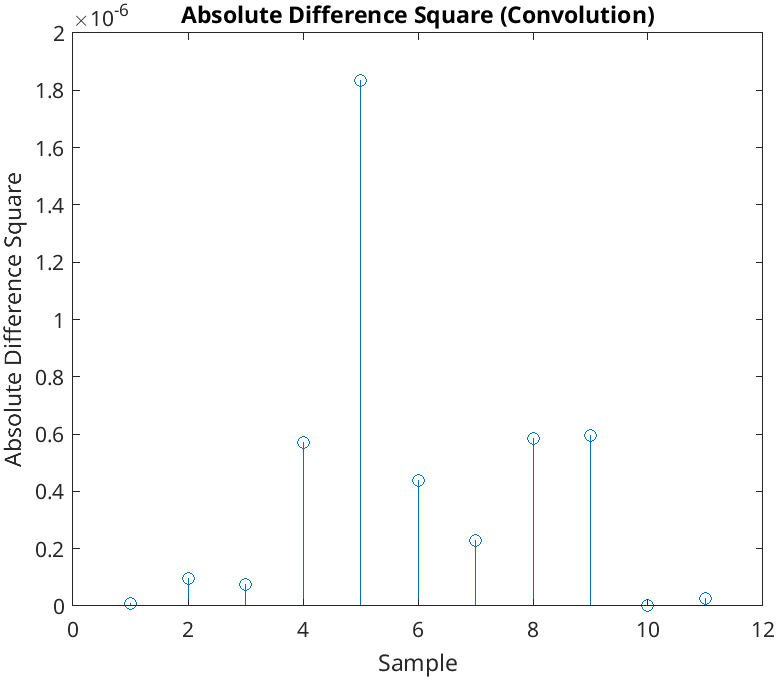
\includegraphics[width=0.8\textwidth]{./figs/conv.png}
    \caption{Square of difference between fixed and floating point convolution}
    \label{fig:convolution}
\end{figure}

\newpage


\subsubsection{Implementation in C}
The fixed point convolution is implemented in C using the same logic as in MATLAB. 
The absolute square difference and mean square error is calculated and printed.

\subsubsection{C Code}
\lstinputlisting[language=C]{../code/convolution.c}

\subsubsection{Output}
\begin{lstlisting}
    fixed convolution:
    0.244771 2.486940 1.203478 -1.465452 7.914201 9.230689 1.321182 2.541230 5.363862 0.928139 -0.088746 
    float convolution:
    0.244856 2.487249 1.203201 -1.466209 7.915555 9.231352 1.320703 2.541995 5.364633 0.928089 -0.088908 
    absolute error Square:
    7.209167e-09 9.577002e-08 7.662044e-08 5.719348e-07 1.833905e-06 4.393087e-07 2.291963e-07 5.853554e-07 5.952470e-07 2.506795e-09 2.607464e-08 
    mean square: 4.057389e-07
\end{lstlisting}

\subsection{Correlation}
Correlation is a statistical measure that expresses the extent to which two variables are linearly related.
The correlation coefficient is a value that indicates the strength and direction of the relationship between variables.
In discrete time, the correlation of two sequences is given by
\[
    r[k] = \sum_{n=-\infty}^{\infty} x[n]h[n+k]
\]

\subsubsection{Implementation in MATLAB}
The fixed point correlation is implemented in MATLAB using the same logic as in the convolution,
but the correlation function is used instead of the convolution function. The 
difference in both the functions is that the second sequence is not flipped before the correlation operation.
The absolute square difference and mean square error is calculated and printed.
The absolute square of the difference between the fixed and floating point results is plotted.


\subsubsection{Matlab Code}
\lstinputlisting[language=Matlab]{../code/correlation.m}

\subsubsection{Output}
\begin{lstlisting}
    fixed correlation:
    0.4826    5.5519    9.1893    1.7090    1.4334    7.6994    2.8707   -1.7700    2.0278    0.5312   -0.0450

    float correlation:
        0.4827    5.5523    9.1903    1.7093    1.4328    7.7005    2.8711   -1.7710    2.0282    0.5314   -0.0451

    absolute error Square:
       1.0e-05 *

        0.0015    0.0200    0.1118    0.0046    0.0309    0.1173    0.0160    0.0925    0.0127    0.0022    0.0007

    mean square : 
       3.7289e-07
\end{lstlisting}

\begin{figure}[h]
    \centering
    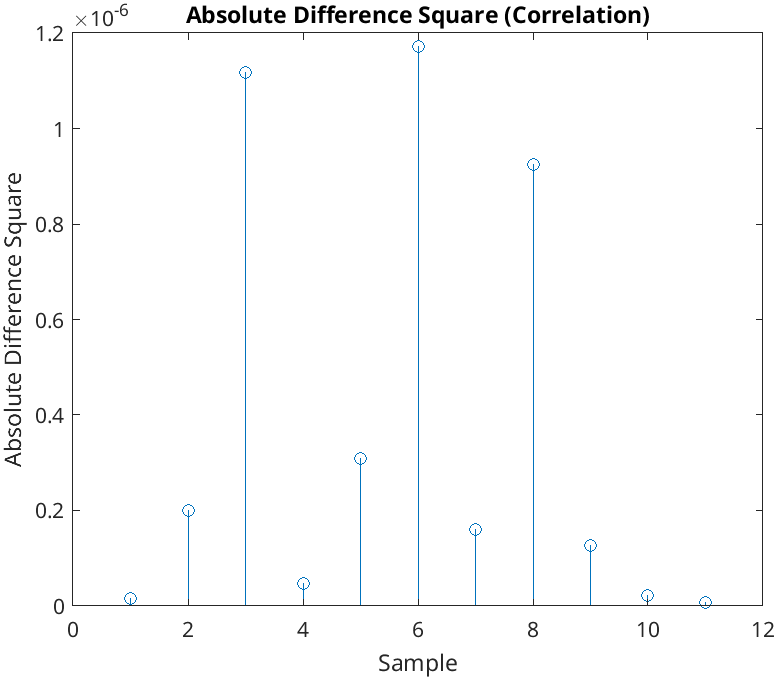
\includegraphics[width=0.8\textwidth]{./figs/corr.png}
    \caption{Square of difference between fixed and floating point correlation}
    \label{fig:correlation}
\end{figure}

\newpage

\subsubsection{Implementation in C}
The fixed point correlation is implemented in C using the same logic as in MATLAB.
The absolute square difference and mean square error is calculated and printed.

\subsubsection{C Code}

\lstinputlisting[language=C]{../code/correlation.c}

\subsubsection{Output}
\begin{lstlisting}
    fixed correlation:
    0.482602 5.551889 9.189254 1.709038 1.433385 7.699375 2.870709 -1.769989 2.027810 0.531231 -0.045011 
    float correlation:
    0.482723 5.552337 9.190310 1.709254 1.432830 7.700457 2.871109 -1.770950 2.028167 0.531379 -0.045098 
    absolute error Square:
    1.480672e-08 2.000534e-07 1.116554e-06 4.629932e-08 3.084648e-07 1.170602e-06 1.598624e-07 9.247925e-07 1.272165e-07 2.183299e-08 7.425216e-09 
    mean square: 3.725372e-07
\end{lstlisting}

\section{Observations}
\begin{itemize}
    \item The absolute square of the difference between the fixed and floating point results is plotted in Figure \ref{fig:convolution} and Figure \ref{fig:correlation}.
    \item From the plot, it is clear that the difference between the fixed and floating point results is very small, but peaks at certain points.
    \item This is because the fixed point representation has a limited range and precision, and the rounding, truncation and overflow errors accumulate over time and cause the error to increase at certain points.
    \item The mean square error is also very small, which indicates that the fixed point implementation is very close to the floating point implementation.
    \item The C and MATLAB implementations give the same results, which indicates that the fixed point implementation is consistent across different programming languages.
\end{itemize}

\section{Conclusion}

Finally, we can conclude that the fixed point implementation of convolution and correlation is very close to the floating point implementation, with a very small mean square error. This shows that fixed point 
implementation is a good approximation of floating point implementation, and can be used in applications where floating point arithmetic is not feasible.
Even though floating-point processing can represent a wider range of numbers and is more precise than fixed-point processing, fixed-point processing is less expensive and easier to develop for.

\end{document}